\documentclass{article}
\usepackage[latin1]{inputenc}
\usepackage[T1]{fontenc}
\usepackage{times}
\usepackage{mathtime}
\usepackage{url}
\usepackage{amsmath}
\usepackage{alltt}
\usepackage[dvips]{graphics}
\begin{document}
 
\section{Name }
\textsc{melting} - nearest-neighbor computation of nucleic acid hybridation
\section{Synopsis}
\textbf{melting} [\textit{options }]  
\section{Description }

\textsc{melting} computes, for a nucleic acid duplex, the enthalpy and the
entropy of the helix-coil transition, and then its melting temperature. Three
types of hybridisation are possible: DNA/DNA, DNA/RNA, and RNA/RNA. The program
uses the method of nearest-neighbors. The set of thermodynamic parameters can be
easely changed, for instance following an experimental breakthrough. Melting is
a free program in both sense of the term. It comes with no cost and it is
open-source. In addition it is coded in ISO C and can be compiled on any
operating system. Some perl scripts are provided to show how melting can be used
as a block to construct more ambitious programs.

If you use \textsc{melting}, please quote

\begin{quote}
  Le Nov\`ere. \textsc{melting}, a free tool to compute the
    melting temperature of nucleic acid duplex. \emph{Bioinformatics}, 17: 1226-1227. 
\end{quote}

\section{Options }

The options are treated sequentially. If there is a conflict between the value
of two options, the latter normally erases the former.

\begin{description}
\item [\textbf{-A}\textit{file.nn}] \mbox{}\\
  Informs the program to use \textit{file.nn} as an alternative set of
  nearest-neighbor parameters, rather than the default for the specified
  hybridisation type (option \textbf{-H}). The standard distribution of melting
  provides some files ready-to-use: \textit{all97a.nn} (Allawi et al 1997),
  \textit{bre86a.nn} (Breslauer et al 1986), \textit{san96a.nn} (SantaLucia et
  al 1996), \textit{sug96a.nn} (Sugimoto et al 1996), \textit{san04a.nn} (Santalucia 
  et al 2004)(DNA/DNA),
  \textit{fre86a.nn} (Freier et al 1986), \textit{xia98a.nn} (Xia et al 1998)
  (RNA/RNA) and \textit{sug95a.nn} (Sugimoto et al 1995) (DNA/RNA). The program
  will look for the file in a directory specified during the installation.
  However, if an environment variable NN\_PATH is defined, melting will search
  in this one first. Be careful, the option \textbf{-A } changes the default
  parameter set defined by the option \textbf{-H.}
\item [\textbf{-C}\textit{complementary\_sequence}] \mbox{}\\
  Enters the complementary sequence, from 3' to 5'. This option is mandatory if
  there are mismatches between the two strands. If it is not used, the program
  will compute it as the complement of the sequence entered with the option
  \textbf{-S}
\item [\textbf{-D}\textit{dnadnade.nn}]\mbox{}\\
  Informs the program to use the file \textit{dnadnade.nn} to compute the
  contribution of dangling ends to the thermodynamic of helix-coil transition.
  The dangling ends are not taken into account by the approximative mode.
\item [\textbf{-F}\textit{factor}  ]\mbox{}\\
  This is the a correction factor used to modulate the effect of the nucleic
  acid concentration in the computation of the melting temperature. See section
  ALGORITHM for details.
\item [\textbf{-G}\textit{x.xxe-xx}  ]\mbox{}\\
  Magnesium  concentration  (No maximum concentration for the moment). The effect  
  of  ions  on  thermodynamic  stability  of nucleic  acid duplexes is complex,
  and the correcting functions are  at  best rough  approximations.The published 
  Tm  correction formula for divalent Mg2 ions of  Owczarzy  (2008) can
  take in account the competitive binding of monovalent and divalent ions on DNA. 
  However this formula is only for DNA duplexes.
\item [\textbf{-h}]\mbox{}\\ 
Displays a short help and quit with EXIT\_SUCCESS. 
\item [\textbf{-H}\textit{hybridisation\_type}]\mbox{}\\
  Specifies the hybridisation type. This will set the nearest-neighbor set to
  use if no alternative set is provided by the option \textbf{-A} (remember the
  options are read sequentially). Moreover this parameter determines the
  equation to use if the sequence length exceeds the limit of application of the
  nearest-neighbor approach (arbitrarily set up by the author). Possible values
  are \textit{dnadna}, \textit{dnarna} and \textit{rnadna} (synonymous), and
  \textit{rnarna}. For reasons of compatibility the values of the previous
  versions of melting \textit{A,B,C,F,R,S,T,U,W} are still available although
  \textbf{strongly } deprecated. Use the option \textbf{-A} to require an
  alternative set of thermodynamic parameters. \textbf{Important:} If the duplex
  is a DNA/RNA heteroduplex, the sequence of the DNA strand has to be entered
  with the option \textbf{-S}
\item [\textbf{-I}\textit{input\_file}  ]\mbox{}\\ 
Provides the name of an input file containing the parameters of the
run. The input has to contain one parameter per line, formatted as in
the command line. The order  is not important, as well as blank lines.
example:   

\begin{verbatim}
 -Hdnadna  
 -Asug96a.nn
 -SAGCTCGACTC
 -CTCGAGGTGAG
 -N0.2
 -P0.0001 
 -v 
 -Ksan96a 

\end{verbatim}

\item [\textbf{-i}\textit{file.nn}] \mbox{}\\ 
Informs  the  program to use file.nn as an alternative set  of  inosine pair 
 parameters, rather than  the  default  for the specified hybridisation type. 
 The standard distribution of melting provides some  files ready-to-use:  san05a.nn 
(Santalucia et al 2005) for deoxyinosine in DNA duplexes, bre07a.nn (Brent M Znosko 
 et al 2007)for inosine in RNA duplexes. Note  that  not all the inosine mismatched 
 wobble's pairs have been investigated. Therefore it could be impossible to  compute
 the Tm of a duplex with inosine pairs. Moreover, those inosine pairs are not taken 
 into account by the  approximative mode.
\item [\textbf{-K}\textit{salt\_correction}]\mbox{}\\ 
Permits to chose another correction for the concentration in sodium. Currently, 
one can chose between \textit{wet91a, san96a, san98a}.  See section ALGORITHM 
\item [\textbf{-k}\textit{x.xxe-xx}]\mbox{}\\ 
 Potassium  concentration  (No maximum concentration for the moment). The effect of ions 
 on  thermodynamic  stability  of nucleic  acid duplexes is complex, and the correcting 
 functions are  at  best rough  approximations.The published  Tm  correction formula for 
 sodium ions of Owczarzy (2004)is therefore also applicable to buffers containing Tris or
 KCl. Monovalent K+, Na, Tris+ ions  stabilize  DNA duplexes 
 with similar potency, and their effects on duplex stability are additive. However this formula 
 is only for DNA duplexes.
\item [\textbf{-L}]\mbox{}\\ Prints the legal informations and quit
  with EXIT\_SUCCESS. 
\item [\textbf{-M}\textit{dnadnamm.nn}]\mbox{}\\ 
Informs the program to use the file  \textit{dnadnamm.nn} to compute
the contribution of mismatches to the thermodynamic of helix-coil
transition. Note that not all the mismatched Crick's pairs have been
investigated. Therefore it could be impossible to compute the Tm of a
mismatched duplex. Moreover, those mismatches are not taken into
account by the approximative mode. 
\item [\textbf{-N}\textit{x.xxe-xx}  ]\mbox{}\\
  Sodium concentration (between 0 and 10 M). The effect of ions on thermodynamic
  stability of nucleic acid duplexes is complex, and the correcting functions
  are at best rough approximations. Moreover, they are generally reliable only
  for $[\mbox{Na}^+]$ belonging to [0.1,1~M]. If there are no other ions in 
  solution, we can use only the sodium correction. In the other case, we use the Owczarzy's 
  algorithm..
\item [\textbf{-O}\textit{output\_file}]\mbox{}\\ 
The output is directed to this file instead of the standard
output. The name of the file can be omitted. An automatic name is then
generated, of the form  meltingYYYYMMMDD\_HHhMMm.out (of course, 
on POSIX compliant systems, you  can emulate this with the redirection 
of stdout to a file constructed with the program date).  
\item [\textbf{-P}\textit{x.xxe-xx}]\mbox{}\\ 
Concentration of the nucleic acid strand in excess (between 0 and 0.1 M).
\item [\textbf{-p}]\mbox{}\\ 
Return the directory supposed to contain the sets of calorimetric parameters and quit with
EXIT\_SUCCESS. If the environment variable NN\_PATH is set, it is returned. Otherwise, the value
defined by default during the compilation is returned.
\item [\textbf{-q}  ]\mbox{}\\ 
Turn off the interactive correction of wrongly entered
parameter. Useful for run through a server, or a batch script. Default
is OFF (i.e. interactive on). The switch works in both sens. 
 Therefore if  \textbf{-q } has been set in an input file, another
 \textbf{-q } on the command line will switch the quiet mode OFF (same
 thing if two \textbf{-q } are set on the same command line).  
\item [\textbf{-S}\textit{sequence}  ]\mbox{}\\ 
Sequence of one strand of the nucleic 
acid duplex, entered 5' to 3'. \textbf{Important:} If it is a DNA/RNA  heteroduplex, 
the sequence of the DNA strand has to be entered.  
Uridine and thymidine are 
considered as identical. The bases can be upper or lowercase.
\item [\textbf{-T}\textit{xxx}  ]\mbox{}\\ 
Size threshold before approximative computation. The nearest-neighbour approach 
will be used only if the length of the sequence is inferior to this threshold.
\item [\textbf{-t}\textit{x.xxe-xx}  ]\mbox{}\\ 
Tris buffer  concentration  (No maximum concentration for the moment). 
The effect  of  ions  on  thermodynamic  stability  of nucleic  acid 
duplexes is complex, and the correcting functions are  at  best
rough  approximations.The published  Tm  correction formula for sodium ions of 
Owczarzy (2004)is therefore also applicable to buffers containing Tris or
KCl. Monovalent Monovalent K+, Na, Tris+ ions  stabilize  DNA duplexes with similar potency, and 
their effects on duplex stability are additive. However this formula is only for DNA 
duplexes. Be aware, the $[\mbox{Tris}^+]$ is about half of the total tris buffer
concentration.
\item [\textbf{-v}  ]\mbox{}\\ 
Control the verbose 
mode, issuing a lot more information about the current run  (try it once 
to see if you can get something interesting). Default is OFF. The  switch 
works in both sens. Therefore if  \textbf{-v } has been set in an input file, another 
\textbf{-v } on the command line will switch the verbose mode OFF (same thing if 
two  \textbf{-v } are set on the same command line).  
\item [\textbf{-V}  ]\mbox{}\\ 
Displays the version number 
and quit with EXIT\_SUCCESS 
\item [\textbf{-x}  ]\mbox{}\\ Force the program to compute an approximative 
tm, based on G+C content. This option has to be used with caution. Note 
that such a calcul is increasingly incorrect when the length of  the duplex 
decreases. Moreover, it does not take into account nucleic acid concentration, 
which is a strong mistake.    
  
\end{description}
 
\section{Algorithm }
  
   
\subsection{Thermodynamics of helix-coil transition of nucleic acid}  
The nearest-neighbor approach is based on the fact that the helix-coil
transition works as a zipper. After an initial attachment, the hybridisation
propagates laterally.  Therefore, the process depends on the adjacent
nucleotides on each strand (the Crick's pairs).  Two duplexes with the same base
pairs could have different stabilities, and on the contrary, two duplexes with
different sequences but identical sets of Crick's pairs will have the same
thermodynamics properties (see Sugimoto et al. 1994).  This program first
computes the hybridisation enthalpy and entropy from the elementary parameters
of each Crick's pair.
\begin{displaymath}
  \begin{array}[t]{ccc}
  \Delta{}H&=&\delta{}h_\mathrm{initiation}+\sum \delta{}h_\mathrm{Crick's pair}\\
  \Delta{}S&=&\delta{}s_\mathrm{initiation}+\sum \delta{}s_\mathrm{Crick's pair}
  \end{array}
\end{displaymath}
   
See Wetmur J.G. (1991) and SantaLucia (1998) 
for deep reviews on the nucleic  acid hybridisation and on the different 
set of nearest-neighbor parameters.    

\begin{figure}[h]
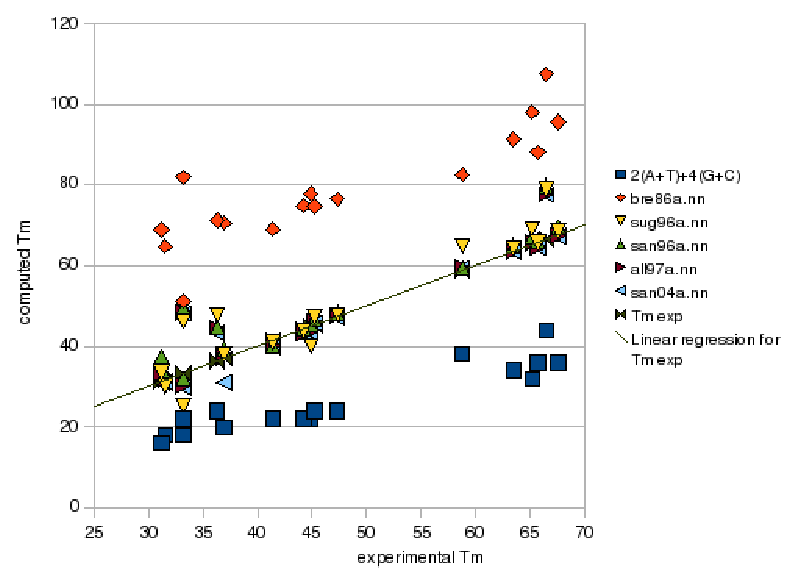
\includegraphics{image1M.eps}
\caption{Comparison of experimental and computed Tm for various sets of
  nearest-neighbor parameters. $[\mbox{Na}^+] = 1$~M, $[\mbox{nucleic acid}] = 4\cdot{}10^{-4}$~M}
\end{figure}

\begin{figure}[h]
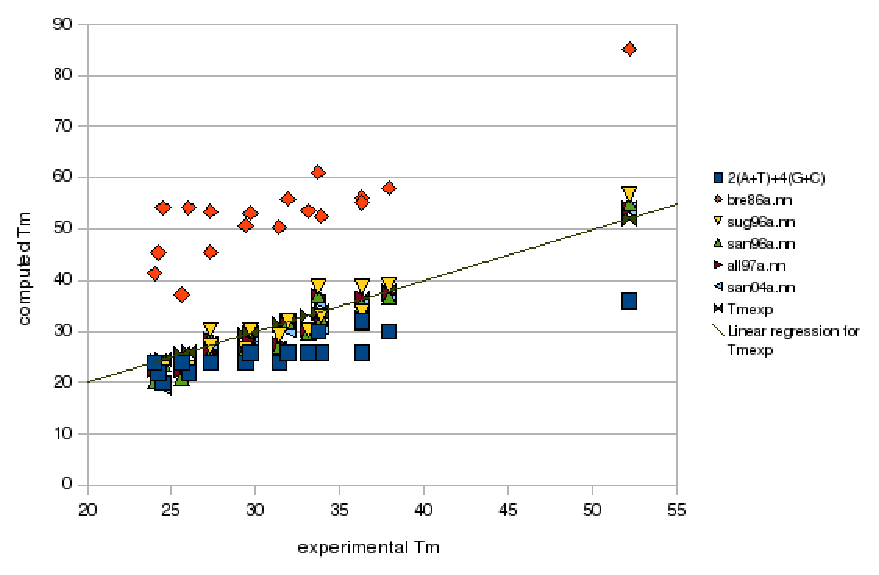
\includegraphics{image0_11M.eps}
\caption{Comparison of experimental and computed Tm for various sets of
  nearest-neighbor parameters. $[\mbox{Na}^+] = 0.11$~M, $[\mbox{nucleic acid}] = 8\cdot{}10^{-6}$~M}
\end{figure}
   
\subsection{Effect of mismatches and dangling ends}  

The mismatching pairs (inosine  mismatches  included) are also taken into account. However the thermodynamic
parameters are still not available for every possible cases (notably when both
positions are mismatched). In such a case, the program, unable to compute any
relevant result, will quit with a warning.  The two first and positions cannot
be mismatched. in such a case, the result is unpredictable, and all cases are
possible. for instance (see Allawi and SanLucia 1997), the duplex
\begin{alltt}
A          T  
 \underline{G}TGAGCTCA\underline{T}  
 \underline{T}ACTCGAGT\underline{G}  
T          A   
\end{alltt}

is more stable than 

\begin{alltt}
A\underline{G}TGAGCTCA\underline{T}T 
T\underline{T}ACTCGAGT\underline{G}A 
\end{alltt}
   
The dangling ends, that is the unmatched terminal nucleotides, can be taken into
account.

\subsection{Example}

\begin{multline*}
\Delta H {\mbox{\texttt{AGCGATGAA-}} \choose \mbox{\texttt{-CGCTGCTTT}}} = 
\Delta H {\mbox{\texttt{AG}} \choose \mbox{\texttt{-C}} } + 
\Delta H {\mbox{\texttt{A-}} \choose \mbox{\texttt{TT}} } \\ +
\Delta H {\mbox{\texttt{G}} \choose \mbox{\texttt{C}} }_\mathrm{init} +
\Delta H {\mbox{\texttt{A}} \choose \mbox{\texttt{T}} }_\mathrm{init} \\ +
\Delta H {\mbox{\texttt{GC}} \choose \mbox{\texttt{CG}} } +
\Delta H {\mbox{\texttt{CG}} \choose \mbox{\texttt{GC}} } +
2x \Delta H {\mbox{\texttt{GA}} \choose \mbox{\texttt{CT}} } +
\Delta H {\mbox{\texttt{AA}} \choose \mbox{\texttt{TT}} } \\ +
\Delta H {\mbox{\texttt{A\underline{T}}} \choose \mbox{\texttt{T\underline{G}}} } +
\Delta H {\mbox{\texttt{\underline{T}G}} \choose \mbox{\texttt{\underline{G}C}} }
\end{multline*}

       (The same computation is performed for $\Delta S$)


\subsection{The melting temperature }  
Then the melting temperature is computed by the following formula:   

\begin{tabular}{rcp{1.6in}p{2.2in}}
Tm & = & \begin{math} \frac{\Delta{}H}{\Delta{}S + R \ln (C_T/F)} \hspace{2em} + \end{math} & \begin{math}\mathcal{F}([\mathrm{Na}^+]) - 273.15 \end{math} \\
   &   &                                                                                          &                                                       \\
   &   & \footnotesize \textit{Tm} in K (for [Na$^+$] = 1~M)    &\footnotesize \emph{correction} for the 
salt concentration (if there are only Na+ cations in the solution) and to get the temperature in degree Celsius. (In fact 
some corrections are directly included in the $\Delta S$ see that of SanLucia 
1998)    
\end{tabular}
   
\subsection{Correction for the concentration of nucleic acid }  

\textit{F} is 1 in the case of self-complementarity oligonucleotides. If the
ODNs are not self-complementary, \textit{F} is 4 if both strands are present in
equivalent amount and \textit{F} is 2 if one strand is in excess (for instance
in \textsc{pcr} experiments).  Actually in the latter case, the formula would
have to use the difference of concentrations rather than the total
concentration. But if the excess is sufficient, the total concentration can be
assumed to be identical to the concentration of the strand in excess. That is,
if one strand is in excess, the actual formula is effectively $(C_{\mbox{max}} -
C_{\mbox{min}})/2$ but if $C_{\mbox{max}} \gg C_{\mbox{min}}$, $C_{\mbox{max}}
- C_{\mbox{min}}$ is close to the total concentration $C_T$.  If $C_{\mbox{max}}$ is close
to $C_{\mbox{min}}$, $(C_{\mbox{max}} - C_{\mbox{min}})/2$ is equivalent to $C_T/4$, which is the default
correction.

Note however that \textsc{melting} makes the assumption of no self-assembly,
\textit{i.e.}  the computation does not take any entropic term to correct for
self-complementarity.
  
\subsection{Correction for the concentration of salt }  

If there are only sodium ions in the solution, we can use the following
corrections:  the correction can be chosen between \textit{wet91a,} presented in
Wetmur 1991 \textit{i.e.}
\begin{displaymath}
  16.6  \log \frac{[\mbox{Na}^+]}{1 + 0.7 [\mbox{Na}^+]} + 3.85   
\end{displaymath}

  \textit{san96a} presented in SantaLucia et al. 1996 
\textit{i.e.}  
\begin{displaymath}
12.5  \log [\mbox{Na}^+]   
\end{displaymath}
  and  \textit{san98a} presented in SantaLucia 1998 \textit{i.e.} a correction 
of the entropic term without modification of enthalpy  
\begin{displaymath}
  \Delta{}S=\Delta{}S_{[\mbox{Na}^+]=1\;\mathrm{M}}+0.368 (N-1) \ln [\mbox{Na}^+]   
\end{displaymath}
  Where \emph{N} is the length of the duplex.   
   
\begin{figure}[h]
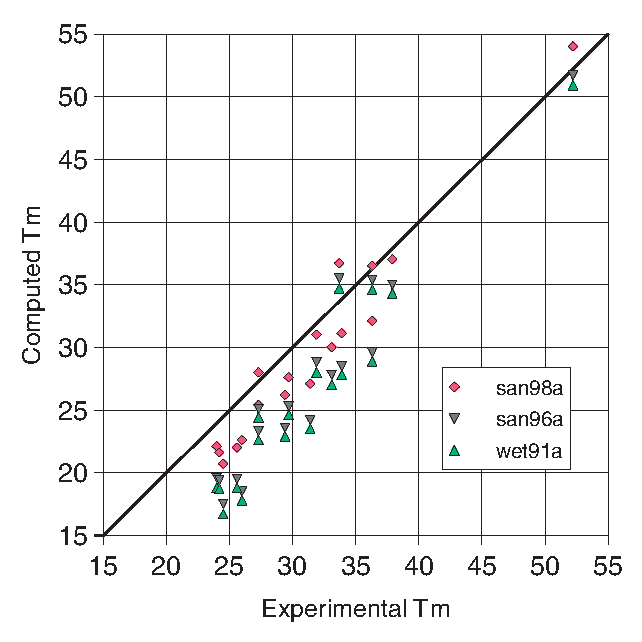
\includegraphics{salt.eps}
\caption{Comparison of experimental and computed Tm for various correction
of salt concentration.}
\end{figure}

\subsection{Correction for the concentration of ions when other monovalent ions such as 
Tris+ and K+ or divalent Mg2+ ions are added}  

If there are only Na+ ions, we can use the correction for the concentration of salt
(see above). In the opposite case, we will use the magnesium and monovalent ions correction
from Owczarzy (2008). (only for DNA duplexes)
\begin{displaymath}
 [\mbox{Mon}^+] = [\mbox{Na}^+] + [\mbox{k}^+] + [\mbox{Tris}^+]
\end{displaymath}
  Where $[\mbox{Tris}^+]$ is equal to half of total tris buffer concentration. (in the option -t, it is the Tris buffer concentration
which is entered).

When the divalent ions are the only ions present, the melting temperature is :
\begin{displaymath}
\frac{1}{Tm_{[\mbox{Mg}^{2+}]}} = \frac{1}{Tm_{[\mbox{Na}^+]=1\;\mathrm{M}}} + a
- b (\ln [\mbox{Mg}^{2+}]) + Fgc (c + d \ln [\mbox{Mg}^{2+}]) + \frac{1}{2 (Nbp-1)} 
\end{displaymath}
\begin{displaymath}
(-e + f \ln [\mbox{Mg}^{2+}] + g (\ln [\mbox{Mg}^{2+}])^{2}])
\end{displaymath}
   where : 
a = 3.92 x $10^{-5}$
b = 9.11 x $10^{-6}$
c = 6.26 x $10^{-5}$
d = 1.42 x $10^{-5}$
e = 4.82 x $10^{-4}$
f = 5.25 x $10^{-4}$
g = 8.31 x $10^{-5}$.

Fgc is the fraction of GC base pairs in the sequence and 
Nbp is the length of the sequence (Number of base pairs).

When there are both monovalent and divalent ions, there are several cases because we can have
a competitive DNA binding between monovalent and divalent 
cations.

If the following ratio :
\begin{displaymath}
  \frac{[\mbox{Mg}^{2+}]^{0.5}]}{[\mbox{Mon}^+]}  
\end{displaymath}
is inferior to 0.22, monovalent ion influence is dominant, divalent cations can be 
disregarded and the melting temperature is :
\begin{displaymath}
\frac{1}{Tm_{[\mbox{Mg}^{2+}]}} = \frac{1}{Tm_{[\mbox{Na}^+]=1\;\mathrm{M}}} + (4.29
Fgc - 3.95)\cdot{}10^{-5} \ln [\mbox{Mon}^+] + 9.40\cdot{}10^{-6} (\ln [\mbox{Mg}^{2+}])^{2})
\end{displaymath}
  
\begin{figure}[H]
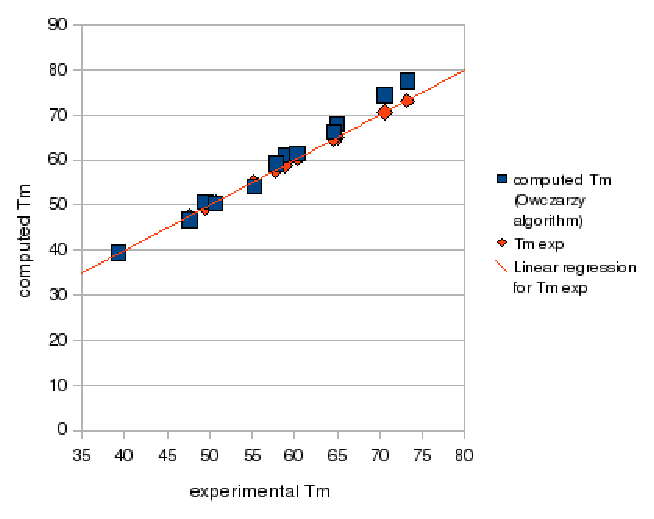
\includegraphics{Owczarzy2.eps}
\caption{Comparison of experimental and computed Tm with the algorithm of Owczarzy (2008). 
$[\mbox{Mon}^+] = 0.055$~M, $[\mbox{Mg}^{2+}] = 0$~M, $[\mbox{nucleic acid}] =
2\cdot{}10^{-6}$~M. The ratio is inferior to 0.22}
\end{figure}


If the ratio is included in [0.22, 6[,we must take in account both Mg2+ and monovalent cations 
concentrations. The melting temperature is calculated with the first equation but with monovalent 
ions concentration dependent parameters a, d and g :

\begin{displaymath}
a = 3.92\cdot{}10^{-5} (0.843 - 0.352 [\mbox{Mon}^+]^{0.5} \ln [\mbox{Mon}^+]) 
\end{displaymath}
\begin{displaymath}
d = 1.42\cdot{}10^{-5} (1.279 - 4.03\cdot{}10^{-3} \ln [\mbox{Mon}^+] -
8.03\cdot{}10^{-3} \ln [\mbox{Mon}^+]^{2})
\end{displaymath}
\begin{displaymath}
g = 8.31\cdot{}10^{-5} (0.486 - 0.258 \ln [\mbox{Mon}^+] + 5.25\cdot{}10^{-3}
\ln [\mbox{Mon}^+]^{3} 
\end{displaymath}

\begin{figure}[H]
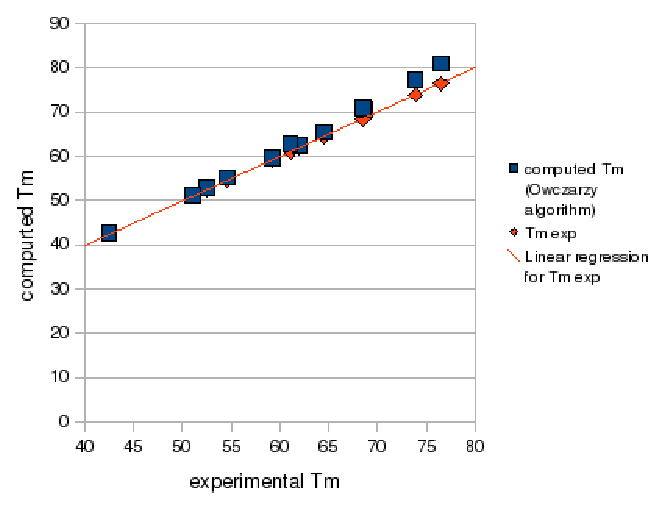
\includegraphics{Owczarzy3.eps}
\caption{Comparison of experimental and computed Tm with the algorithm of Owczarzy (2008). 
$[\mbox{Mon}^+] = 0.055$~M, $[\mbox{Mg}^{2+}] = 0.0015$~M, $[\mbox{nucleic acid}] =
2\cdot{}10^{-6}$~M. The ratio is included in [0.22, 6[.}
\end{figure}

Finally, if the ratio is superior to 6,divalent ion influence is dominant, monovalent cations can be 
disregarded and the melting temperature is calculated with the first equation and the constant parameters a, b, c, d,
e, f, g.

\begin{figure}[H]
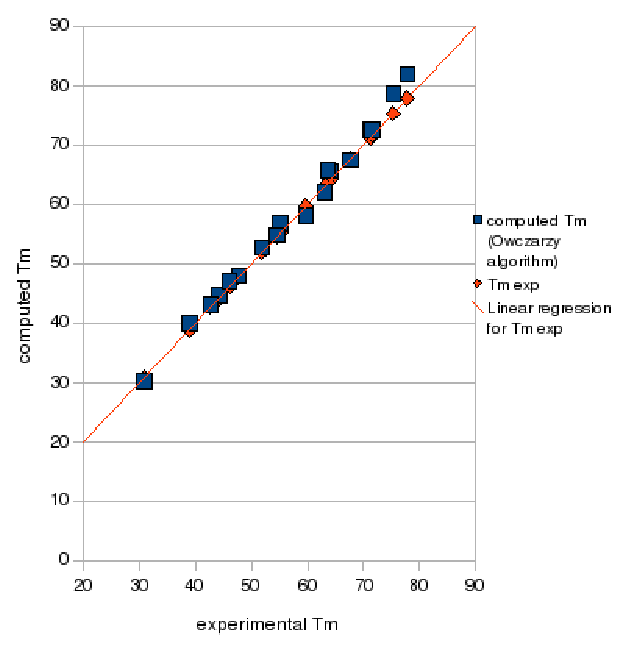
\includegraphics{Owczarzy1.eps}
\caption{Comparison of experimental and computed Tm with the algorithm of Owczarzy (2008). 
$[\mbox{Mon}^+] = 0.001$~M, $[\mbox{Mg}^{2+}] = 0.0015$~M, $[\mbox{nucleic acid}] =
2\cdot{}10^{-6}$~M. The ratio is superior to 6.}
\end{figure}
    
\subsection{Long sequences }  
  It is important to realise that the nearest-neighbor approach 
has been established  on small oligonucleotides. Therefore the use of \textsc{melting} 
in the non-approximative  mode is really accurate only for relatively short 
sequences (Although if the sequences are two short, let's say $<$ 6~bp, the 
influence of extremities becomes too important and the  reliability decreases 
a lot). For long sequences an approximative mode has been designed. This mode is 
launched if the sequence length is higher than the value 
given by the option -T (the default threshold is 60 bp).
 
The melting temperature is computed by the following formulas:   

\textsc{adn/adn}:
\begin{displaymath}
Tm = 81.5 + 16.6\log\frac{[\mbox{Na}^+]}{1+0.7[\mbox{Na}^+]} + 0.41\% GC - \frac{500}{size}
\end{displaymath}
\textsc{adn/arn}:
\begin{displaymath}
Tm = 67 + 16.6\log\frac{[\mbox{Na}^+]}{1+0.7[\mbox{Na}^+]} + 0.8\% GC - \frac{500}{size}
\end{displaymath}
\textsc{arn/arn}:
\begin{displaymath}
Tm = 78 + 16.6\log\frac{[\mbox{Na}^+]}{1+0.7[\mbox{Na}^+]} + 0.7\% GC - \frac{500}{size}
\end{displaymath}

  The usage of this mode is nevertheless  \textbf{strongly disencouraged.}   
   
\subsection{Miscellaneous comments }  
\textsc{melting} is currently accurate only when the hybridisation is performed
at pH $7\pm 1$.  The computation is valid only for the hybridisations performed
in aqueous medium. Therefore the use of denaturing agents such as formamide
completely invalidates the results.
   
\section{References }
Allawi 
H.T., SantaLucia J. (1997). Thermodynamics and NMR of internal G-T mismatches 
in DNA. \textit{Biochemistry}  36: 10581-10594   

Allawi H.T., SantaLucia J. (1998). Nearest Neighbor thermodynamics parameters 
for internal G.A mismatches in DNA. \textit{Biochemistry} 37: 2170-2179

Allawi H.T., SantaLucia J. (1998).Thermodynamics of internal C.T mismatches in DNA.
\textit{Biochemistry} 26: 2694-2701.

Allawi H.T., SantaLucia J. (1998). Nearest Neighbor thermodynamics of internal 
A.C mismatches in DNA: sequence dependence and pH effects.
\textit{Biochemistry} 37: 9435-9444.

Bommarito S., Peyret N., SantaLucia J. (2000).  Thermodynamic parameters for DNA
sequences with dangling ends.  \textit{Nucleic Acids Res} 28: 1929-1934

  Breslauer K.J., Frank R., Bl\"ocker 
H., Marky L.A. (1986). Predicting DNA duplex stability from the base sequence. 
 \textit{Proc Natl Acad Sci USA}  83: 3746-3750   

  Freier S.M., Kierzek R., Jaeger 
J.A., Sugimoto N., Caruthers M.H., Neilson T., Turner D.H. (1986). \textit{Biochemistry} 
 83:9373-9377 
 
 Owczarzy R., Moreira B.G., You Y., Behlke M.B., Walder J.A.(2008) Predicting stability of DNA duplexes 
 in solutions containing Magnesium and Monovalent Cations. \textit{Biochemistry} 47: 5336-5353.  

Peyret N., Seneviratne P.A., Allawi H.T., SantaLucia J. (1999). Nearest Neighbor thermodynamics and 
NMR of DNA sequences with internal A.A, C.C, G.G and T.T mismatches. dependence and pH effects.
\textit{Biochemistry} 38: 3468-3477

  SantaLucia J. Jr, Allawi H.T., Seneviratne P.A. (1996). Improved 
nearest-neighbor parameters for predicting DNA duplex stability. \textit{Biochemistry} 
35: 3555-3562   

  Sugimoto N., Katoh M., Nakano S., Ohmichi T., Sasaki M. (1994). 
RNA/DNA hybrid duplexes with identical nearest-neighbor base-pairs hve identical 
stability. \textit{FEBS Letters} 354: 74-78   

  Sugimoto N., Nakano S., Katoh M., Matsumura 
A., Nakamuta H., Ohmichi T., Yoneyama M., Sasaki M. (1995). Thermodynamic parameters 
to predict stability of RNA/DNA hybrid duplexes. \textit{Biochemistry} 34: 11211-11216 
  
  Sugimoto N., Nakano S., Yoneyama M., Honda K. (1996).  Improved thermodynamic 
parameters and helix initiation factor to predict stability of DNA duplexes. 
\textit{Nuc Acids Res}  24: 4501-4505  

Watkins N.E., Santalucia J. Jr. (2005). Nearest-neighbor thermodynamics of deoxyinosine 
pairs in DNA duplexes. \textit{Nuc Acids Res} 33: 6258-6267 

Wright D.J., Rice J.L., Yanker D.M., Znosko B.M. (2007). Nearest neighbor parameters for 
inosine-uridine pairs in RNA duplexes. \textit{Biochemistry} 46: 4625-4634

  Xia T., SantaLucia J., Burkard M.E., Kierzek 
R., Schroeder S.J., Jiao X., Cox C., Turner D.H. (1998). Thermodynamics parameters 
for an expanded nearest-neighbor model for formation of RNA duplexes with 
Watson-Crick base pairs. \textit{Biochemistry}  37: 14719-14735   

  For review see: 
  
  SantaLucia J. (1998) A unified view of polymer, dumbbell, and oligonucleotide 
DNA nearest-neighbor thermodynamics. \textit{Proc Natl Acad Sci USA}  95: 1460-1465 

SantaLucia  J., Hicks Donald (2004) The Thermodynamics of DNA structural motifs. 
\textit{Annu. Rev. Biophys. Struct} 33: 415-440 
  
  Wetmur J.G. (1991) DNA probes: applications of the principles of nucleic 
acid hybridization. \textit{Crit Rev Biochem Mol Biol} 26: 227-259   
   
\section{Files }
\begin{itemize}
\item [\textit{*.nn}] Files containing the nearest-neighbor parameters, enthalpy and entropy, 
for each Crick's pair.  They have to be placed in a directory defined during 
the compilation or targeted by the  environment variable NN\_PATH.  
\item [\textit{tkmelting.pl}] A Graphical User Interface written in perl/tk is available for users
who prefer  the 'button and menu' approach.  
\item [\textit{*.pl}] Scripts are available to 
use \textsc{melting} iteratively. For instance, the script multi.pl permits to predict 
the Tm of several duplexes in one shot. The script profil.pl allow
an interactive computation along a sequence, by sliding a window of specified width. 
  
\end{itemize}
 
\section{See Also }
New versions and 
related material can be found at \url{http://www.pasteur.fr/recherche/unites/neubiomol/meltinghome.html} 
and at \url{https://sourceforge.net/projects/melting/}
  
You can use \textsc{melting} through a web server at \url{http://bioweb.pasteur.fr/seqana
l/interfaces/melting.html}
  
\section{Known Bugs }
The infiles have to be ended by a blank line because otherwise the last line is not decoded.

If an infile is called, containing the 
address of another input file, it does not care of this latter.  If it 
is its own address, the program quit (is it a bug or a feature?).   
 
In interactive mode, a sequence can be entered on several lines with a backslash\\
\texttt{AGCGACGAGCTAGCCTA{\textbackslash}\\
AGGACCTATACGAC}\\
If by mistake it is entered as  \\
\texttt{AGCGACGAGCTAGCCTA{\textbackslash}{}AGGACCTATACGAC}

The backslash will be considered 
 as an illegal character. Here again, I do not think it is actually a bug 
(even if it is unlikely, there is a small probability that the  backslash 
could actually be a mistyped base).   
   
\section{Copyright }
Melting is copyright 
\copyright 1997, 2009 by Nicolas Le Nov\`ere and Marine Dumousseau.  

This program is free software; 
you can redistribute it and/or modify it under the terms of the GNU General 
Public License as published by the Free Software Foundation; either version 
2 of the License, or (at your option) any later version.   
  This program 
is distributed in the hope that it will be useful, but WITHOUT ANY WARRANTY; 
without even the implied warranty of MERCHANTABILITY or FITNESS FOR A 
PARTICULAR PURPOSE.  See the GNU General Public License for more details. 
  
  You should have received a copy of the GNU General Public License 
along with this program; if not, write to the Free Software Foundation, 
Inc., 59 Temple Place, Suite 330, Boston, MA  02111-1307 USA   
   
\section{Acknowledgements}
Nicolas Joly is an efficient and kind debugger and advisor.  Catherine
Letondal wrote the HTML interface to melting. Thanks to Nirav Merchant,
Taejoon Kwon, Leo Schalkwyk, Mauro Petrillo, Andrew Thompson, Wong Chee Hong, Ivano
Zara for their bug fixes and comments. Thanks to Richard Owczarzy for his magnesium correction. Finally thanks to the usenet
helpers, particularly Olivier Dehon and Nicolas Chuche.

   
\section{Authors }
Nicolas Le Nov\`ere and Marine Dumousseau, \\
EMBL-EBI, 
Wellcome-Trust Genome Campus
Hinxton Cambridge, CB10 1SD, UK
lenov@ebi.ac.uk
  
\section{History }

See the file ChangeLog for the changes of the versions 4 and more recent.

\end{document}
